\documentclass{article}

\usepackage{amsmath}
\usepackage{amssymb}
\usepackage{hyperref}
\usepackage{indentfirst}
\usepackage{matlab-prettifier}
\usepackage[shortlabels]{enumitem}
\usepackage{graphicx}
\usepackage{physics}
\usepackage[margin=1in]{geometry}

%User defined commands
\newcommand{\inv}[1]{#1^{-1}}
\newcommand{\cond}{\kappa_{||\cdot||}}

\begin{document}
\begin{center}
	\huge{\bf Math 170B: Homework 3} \\
	Merrick Qiu
\end{center}

\section*{Problem 1}
Each polynomial is of degree $<= 2$.
Note that $f(1) = 1$ is continuous and $f(2) = \frac{3}{2}$ is continuous.
\[
	f(x) = 
	\begin{cases}
		x & x \in (-\infty, 1] \\
		-\frac{1}{2}(2-x)^2 + \frac{3}{2} & x \in [1,2] \\
		\frac{3}{2} & x \in [2,\infty)
	\end{cases}
\]
Also note that $f'(1) = 1$ is continuous and $f'(2) = 0$ is continuous.
\[
	f'(x) = 
	\begin{cases}
		1 & x \in (-\infty, 1] \\
		2-x & x \in [1,2] \\
		0 & x \in [2,\infty)
	\end{cases}
\]
Thus, the function is a quadratic spline.
\newpage 

\section*{Problem 2}
Evaluating the derivatives yields
\[
	f(x) = 
	\begin{cases}
		a(x-2)^2+b(x-1)^3 & x \in (-\infty, 1] \\
		c(x-2)^2 & x \in [1,3] \\
		d(x-2)^2 + e(x-3)^3 & x \in [3,\infty)
	\end{cases}
\]
\[
	f'(x) = 
	\begin{cases}
		2a(x-2)+3b(x-1)^2 & x \in (-\infty, 1] \\
		2c(x-2) & x \in [1,3] \\
		2d(x-2) + 3e(x-3)^2 & x \in [3,\infty)
	\end{cases}
\]
\[
	f''(x) = 
	\begin{cases}
		2a+6b(x-1) & x \in (-\infty, 1] \\
		2c & x \in [1,3] \\
		2d + 6e(x-3) & x \in [3,\infty)
	\end{cases}
\]

For continuity at the knots,
\[
	a = c \quad c = d
\]
For continuity of the derivatives,
\[
	-2a = -2c \quad 2c = 2d
\]
For continuity of the second derivative 
\[
	2a = 2c \quad 2c = 2d
\]
Thus the function is a cubic spline whenever $a=c=d$.
\newpage 

\section*{Problem 3}
We have that a spline is composed of many polynomial pieces
\[
	S(x) = 
	\begin{cases}
		S_i(x) & x \in [t_i, t_{i+1}] \\
		&\vdots
	\end{cases}
\]
where each piece is a quadratic polynomial 
\[
	S_i(x) = a_ix^2 + b_ix + c_i.
\]
There are $n-1$ equations, which yields a total of $3(n-1)$ unknowns.
Each polynomial must pass through its endpoints so
\[
	S_i(t_i) = a_it_i^2 + b_it_i + c_i = y_i
\]
\[
	S_i(t_{i+1}) = a_it_{i+1}^2 + b_it_{i+1} + c_i = y_{i+1}
\]
which gives $2(n-1)$ equations.

The derivatives in the inner knots must be equal so 
\[
	S_i'(t_{i+1}) = 2a_it_{i+1} + b_i = 2a_{i+1}t_{i+1} + b_{i+1} = S_{i+1}'(t_{i+1})
\]
This yields $n-2$ more equations.

To get the last equation, we can impose that $z_0 = 0$.
\newpage 

\section*{Problem 4}
This problem is similar to Hermite interpolation except the derivatives dont match at $x_0$.
In order so that $l_0(x_0) = 1$ and $l_0(x_i) = l_0'(x_i) = 0$ when $i>0$ it must be that
\[
	l_0(x) = \prod_{i=1}^n \frac{(x-x_i)^2}{(x_0-x_i)^2}
\]
We want that(but only for $j>0$ for the derivative)
\[
	h_i(x_j) = \delta_{ij} \quad \quad h_i'(x_j) = 0.
\]
Let $L_i(x)$ be 
\[
	L_i(x) = \prod_{\substack{j=1 \\ j \neq i}}^n \frac{x-x_j}{x_i-x_j}.
\]
Then we can construct $h_i(x)$ to have the properties we want with
\[
	h_i(x) = \frac{x-x_0}{x_i-x_0}L_k(x)^2[1+C(x-x_i)]
\]
for some constant $C$.
Note that $h_i(x_i) = 1$ and when $i\neq j$, $h_i(x_j) = 0$.
so $h_i(x)$ satisfies our first property.
The derivative is also always $0$
The derivative of $h_i'(x)$ is 
\[
	h_i'(x_i) = \frac{1}{x_i - x_0} + 2L_i'(x_i) +  C =0
\]
so we can set 
\[
	C = -\frac{1}{x_i - x_0} - 2L_i'(x_i).
\]
Similarly we want that 
\[
	k_i(x_j) = 0 \quad \quad k_i'(x_j) = \delta_{ij}.
\]
The polynomial that satisfies these conditions is 
\[
	k_i(x) = \frac{x-x_0}{x_i-x_0}L_k(x)^2(x-x_i)
\]
Note that $h_i(x_i) = 0$ and the derivative is only 1 when $i=j$

Since this polynomial can be thought of as 
interpolation where each point is repeated twice
except for $x_0$, which yields a total of $2n+1$.
By the Lagrange error formula we can write that 
\[
	f(x) - p_{2n}(x) = \frac{(x-x_0)\prod_{i=1}^n (x-x_i)^2}{(2n+1)!}f^{(2n+1)}(\eta)
\]
\newpage 

\section*{Quadratic Spline}
\lstinputlisting[style=Matlab-editor]{QuadFit.m}
\begin{verbatim}
ans =

   -0.6667   -9.3333  -12.6667
    0.3333   -1.3333    3.3333
    0.0000   -2.0000    3.0000
   -0.2500   -2.0000    3.0000
    0.1111   -3.4444    4.4444
   -0.0833   -1.5000   -0.4167
\end{verbatim}
From the matlab code, we can see that the spline for example 6.2 is
\[
	S(x) =
	\begin{cases}
		-\frac{2}{3}x^2 - \frac{28}{3}x - \frac{38}{3} & -7 \leq x \leq -4 \\
		\frac{1}{3}x^2 - \frac{4}{3}x + \frac{10}{3} & -4 \leq x \leq -1 \\
		-2x + 3 & -1 \leq x \leq 0 \\
		-\frac{1}{4}x^2 - 2x + 3 & 0 \leq x \leq 2 \\
		\frac{1}{9}x^2 - \frac{31}{9}x + \frac{40}{9} & 2 \leq x \leq 5 \\
		-\frac{1}{12}x^2 - \frac{3}{2}x - \frac{5}{12} & 5 \leq x \leq 7 \\
	\end{cases}
\]
Plotting this spline, we get 

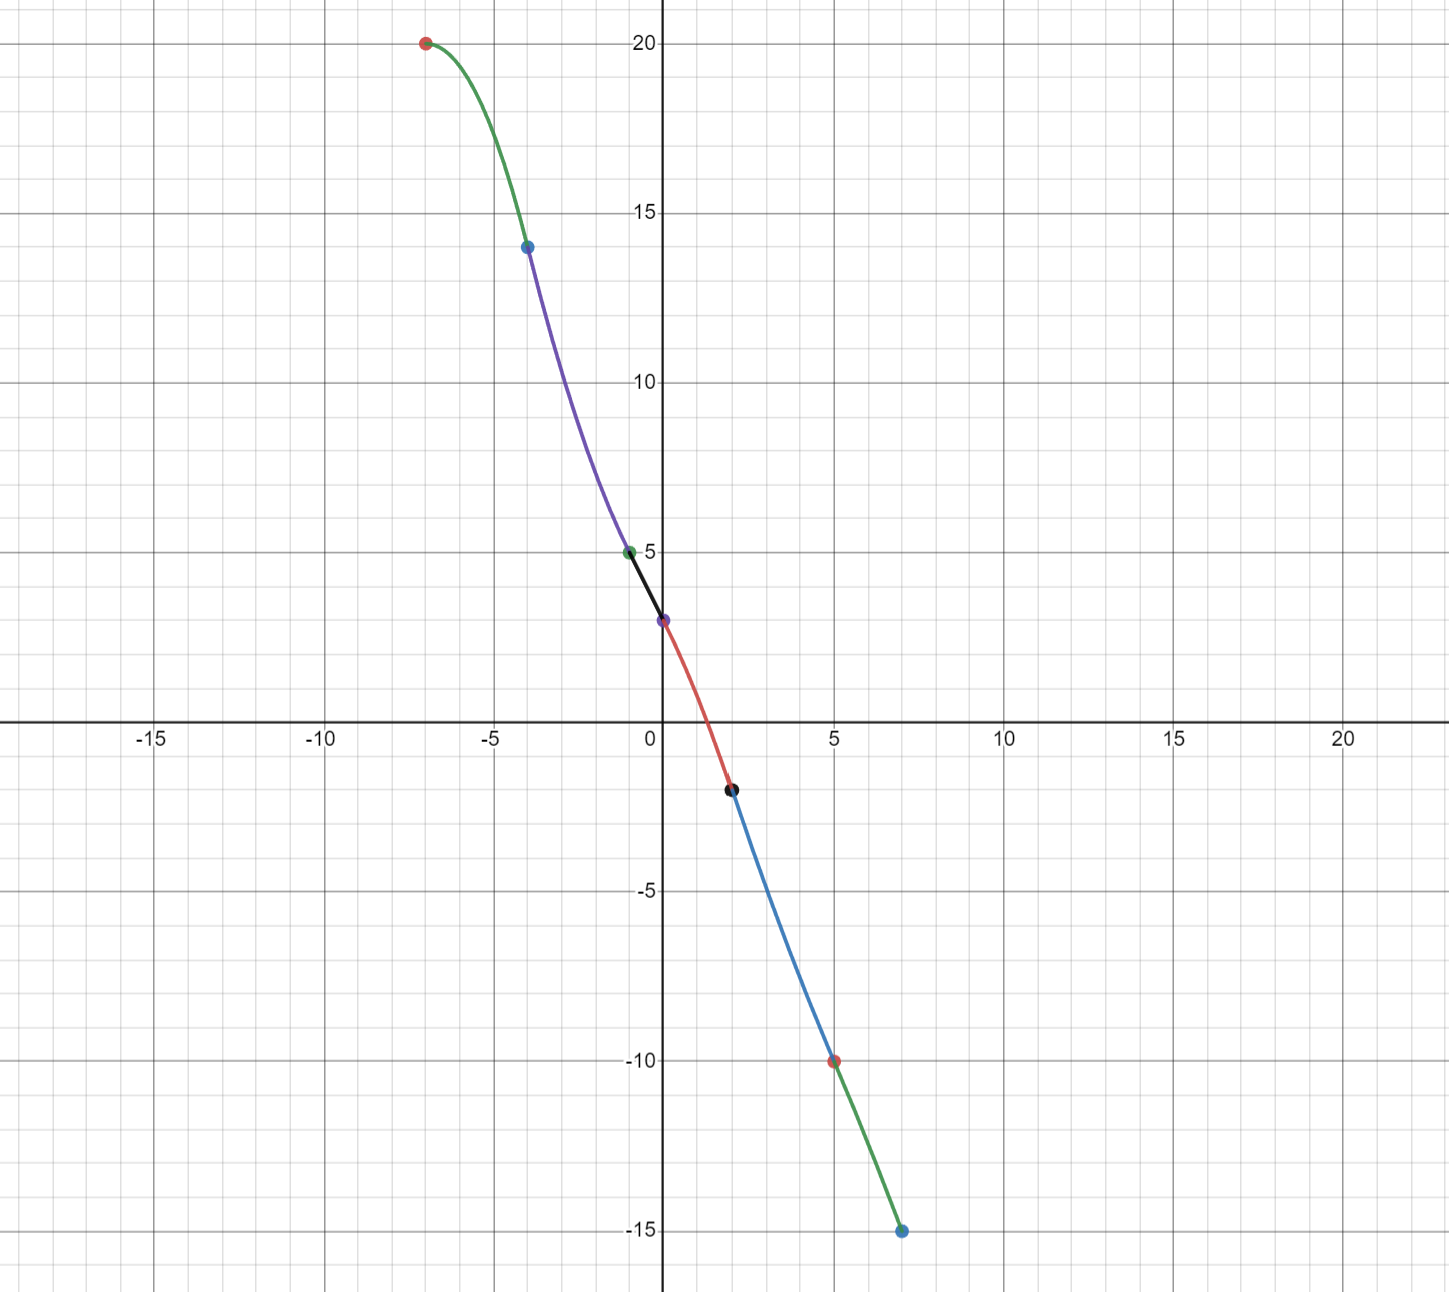
\includegraphics[width=4in]{spline image.png}

\end{document}
